
\begin{abstract}
The abstract should summarize the contents of the paper and should
contain at least 70 and at most 150 words. It should be written using the
\emph{abstract} environment.
\keywords{We would like to encourage you to list your keywords within
the abstract section}
\end{abstract}
%
%-------------------------------------------------------
%
\lyhpi{这个问题可以分三个层次(要不要写进论文?或者可以将related work按照这个来写):\\
	1. Alignment:求解overhead image(的edge image)和3D model的竖直投影对齐,假定相机光轴方向与竖直反向对齐。求解只有一个自由度的R,两个自由度的T和一个scale(相当于T的z方向的自由度)。\\
	2. Geo-localization: 找到相机的6DoF pose。3D orientation and 3D location.\\
	3. 2D-3D registration;求解KRT,K的自由度自定,至少包括$f,u_c,v_c$\\
	以上三个层次都可以另外加入一些distortion,如长宽比,剪切比,偏心扭曲等。\\
	}

\lyhpi{目前我们的算法主要解决的是一个geo-localization的问题,求解camera pose(主要)。然后可以用camera pose来求correspondences (未解决),最后用correspondences来做geo-registration问题(非主要)。}
%
%---------------------- Introduction ---------------------------------
%
\section{Introduction}
%
\paragraph{Background/Motivation}
\lyhpi{一开始提data types是为了方便下面existing methods里面按照data type的不同展开。}
Geo-localization has developed rapidly in recent years with the help of powerful sensors which generate a wide variety of types of data, \xj{such as 3D points, dsm??} 
As a key technique to image-based navigation,augmented reality (AR) and 3D reconstruction, geo-localization in urban outdoor environment has drawn massive attentions in the literature.
%
Geo-localization is more challenging than indoor geo-localization because of more complicated environments~\cite{Arth2015a} with more occlusions, more classes of objects and less regular layouts. \xj{explain why outdoor scene is more complicated? occlusions? more classes of objects? no regular shape?}
 %
 \begin{figure*}[!tp]
 	\centering
 	\vspace{2.0cm}
 	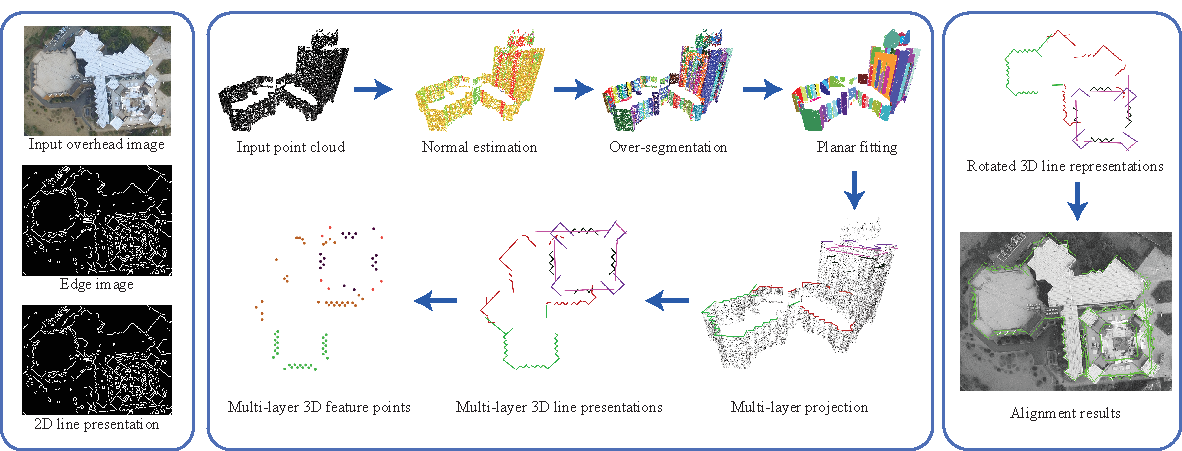
\includegraphics[width=\textwidth]{figures/pipeline_pdf}
 	\caption{Algorithm overview. }
 	\label{fig:overview}
 \end{figure*}
 %
%
\paragraph{Problem statement}
\xj{Do we solve a geo-localization problem?}\lyh{目前paper将问题当做geo-localization问题来解,最后再提及用作初始化解registration问题(这部分没有创新点)}
Outdoor geo-localization aims to compute a large-scale, robust and accurate camera registration in a global coordinate system with metric scale, while it is also different from Simultaneous Localization and Mapping (SLAM) \lyhnew{which does not employ models and therefore presents only relative poses in an arbitrary coordinate system with unknown scale and requires additional motions for initialization \cite{instant}.}
\xj{I don't think this is the key difference. When you say global coordinated system, you just use the 3D model as reference coordinate system. No difference with SLAM. }
\lyh{相比于geo-localzation,SLAM有以下特点:\\
	0. SLAM不需要格外的模型,只要图片/视频,绘制出来的地图是在一个未知的scale下做的。\\
	1. 由于同时做定位和地图绘制,于是定位出来的结果也只是在这个未知scale下的坐标内的位置。\\
	2. 由于是未知坐标,后续为了应用到真实世界,还要在SLAM的基础上加上一个alignment方法才能使用。\\
	3. SLAM要有一个初始化的过程,不然没法自建起一个坐标系统。\\}
\xj{what is the key problem? what is input data and output?}
%
\paragraph{Existing methods and challenges}
When presenting a geo-localization problem, an image or a frame of video is often used as the query data, a 3D model is needed to provide a global coordinate, \lyhnew{a sensor prior is optionally employed, }and the camera pose with respect to the global coordinate system is to be estimated.
\\
\lyhpi{下面这段按照image的不同,简单讨论了现有的方法}\\
%回头确认这几个方法是不是都用了消失点
Some methods capture images or videos by cameras on mobile phones~\cite{Arth2015a, instant, Poglitsch2015, Liu2012} or vehicles~\cite{Taneja2015} on the ground, which are able to take advantages of perspective to compute the camera pose by estimating vanish points. %加一句评价,讲讲消失点很有用
Moreover, some other methods utilize the aerial devices, such as satellites and air plane, to take overhead images at high altitudes, which align the roofs of buildings in images with respect to 3D models (often 3D point clouds), assuming that building roofs in one overhead image captured in high altitude are of a same scale\lyh{有着相同的scale} and therefor projecting 3D models along the vertical vector to generate the global coordinate systems. When it comes to low altitude, perspective effect is more critical, making it a more challenging problem.
\\
\lyhpi{下面这段按照global coordinate system的不同,简单讨论了现有的方法}\\
To obtain the global coordinate system \xj{why to obtain coordinate system?}, some \cite{} maintain databases of pre-registered multiple images. These methods limit themselves while having to collect numerous images covering target areas otherwise only popular spots are available. Another way is employing 3D models, such as digital surface models (DSMs)~\cite{} and 3D point clouds~\cite{}.
\\

\lyhpi{下面提及点云的获得方法和特点来解释为什么要选择用shape matching方法}\\
To acquire 3D point cloud data, a common approach is structure-from-motion (SfM) method\cite{} which is convenient requiring only a series of images to recover a point cloud of a scene. The LiDAR sensor in air plane provides a large-scale but low-quality point cloud\cite{}. 3D models comprising with millions of points can be generated by ground laser scan devices, which provide highly accurate and dense data with metric scaling. However, these laser devices usually fail to capture buildings roof while only vertical facades of buildings are scanned.
\xj{highlight: Missing of roof data makes the registration problem of bird-eye view and 3D models significant challenging.}
\lyh{To be solved}
%
More recently \cite{instant} presents a novel technique that use an untextured 2.5D map (2D map and height) which is \comment{unavailable in some cities and } inaccurate in details.%在很多cities,建筑的2D map都不准确 
\xj{3d models are also unavailable for many cities...}
%
\paragraph{Our key idea and contributions}
\xj{ To solve what problem, we present our method? }
%
In this paper, we present a novel algorithm to \lyhnew{geo-localize the camera of} an overhead image captured by a quadrotor in a low altitude by computing the 6-Dimension-of-Freedom(6DOF) camera pose of the image with respect to the point cloud model coordinate of metric scale. 
%
At first, we treat this problem as a shape matching problem between the edge image of the overhead image and the 2D line presentation of the point cloud \lyhnew{to generate an initial pose for subsequent steps.}
\xj{why use shape matching? what kind of properties will solve the above problem?}
%
We obsolete the high-altitude assumption that building roofs in overhead images are of same scales and propose a novel multi-level strategy to handle low-altitude overhead images where assign different scales to roofs in different heights. 
Moreover, once we achieve the shape matching results we determine the correspondences by matching corners of images with feature points of point clouds. 
At last, we geo-register these two types of data using sparse bundler adjust (SBA) algorithm. 

\lyhnew{\lyhpi{contributions}
To sum up, the contribution of our paper is three-fold. 
At first, we introduce a novel multi-level strategy to handle the low-altitude image. 
Moreover, 
At last,}
